\documentclass[10pt]{article}
\usepackage[margin=1in]{geometry}
\usepackage{booktabs}
\usepackage{graphicx}
\usepackage{amsmath}
\usepackage{amssymb}
\usepackage{microtype}
\usepackage{xcolor}
\usepackage{hyperref}
\usepackage{cleveref}
\usepackage{enumitem}
\usepackage{caption}
\usepackage{subcaption}
\usepackage{array}

\newcommand{\todo}[1]{\textcolor{red}{[TODO: #1]}}
\newcommand{\method}{Urban Visual Gene}
\graphicspath{{../formal/figures/}{../formal/site/}}

\title{Urban Visual Genes: Discovering Reproducible and Interpretable\\
Visual Primitives from Street-Level Imagery}
\author{Ce Hou\\University of California, Berkeley\\\texttt{\todo{email}}
\and \todo{Wenrui Xu, affiliation}
\and \todo{Emma Pierson, affiliation}}
\date{Draft: September 2026}

\begin{document}
\maketitle

\begin{abstract}
Street-view imagery supports measurement of the built environment at scale, but
most existing pipelines either predict a predefined label or return dense features
that are difficult to interpret. We introduce \method, a framework that decomposes
patch-level representations from a frozen DINOv3 vision transformer into sparse,
recurring visual primitives using a BatchTopK sparse autoencoder (SAE). Our main
experiment uses 14,400 directional street-view images from 12 globally distributed
cities, yielding 11.29 million image patches. A 1,024-dimensional dictionary with
eight active genes per patch reconstructs the source representation with approximate
cosine similarity 0.849 while retaining broad dictionary utilization. Across five
independent training runs, we identify 875 gene families present in at least four
runs, including 738 recovered in all five. A language-free multiview analysis
organizes the dictionary into 32 coarse and 64 fine branches using decoder, encoder,
spatial-position, city-distribution, and activation-context evidence. Gene profiles
predict held-out road class with mean balanced accuracy 0.622 under spatial
cross-validation, compared with 0.388 for acquisition and image-quality nuisance
variables alone. Finally, an open-source Qwen3-VL model produces structured concept
descriptions for a stratified pilot of 128 genes. These descriptions are preliminary:
their semantic fidelity has not yet been independently validated. Together, the
results establish a reproducible basis for interpretable, comparative ``visual
genomes'' of cities while exposing important challenges in redundancy, nuisance
features, calibration, and semantic evaluation.
\end{abstract}

\section{Introduction}
Street-level imagery offers a human-scale view of cities and has been used to study
urban form, transportation, vegetation, health, socioeconomic conditions, and
perception \cite{biljecki2021streetview}. Yet common analytical approaches depend on
fixed semantic segmenters or supervised prediction targets. Such methods are useful
when the relevant ontology is known in advance, but they cannot easily discover
recurring visual structure outside that ontology. Conversely, foundation-model
embeddings capture rich visual information but do not directly expose a compact,
human-auditable vocabulary.

We ask whether the visual character of cities can instead be represented through a
shared set of learned primitives. We call a recurring sparse feature a \emph{visual
gene}, and the distribution and co-occurrence of genes within a city its \emph{visual
genome}. The biological metaphor is deliberately limited: genes here are learned
components of a visual representation, not causal or immutable attributes of a city.

Our framework applies a sparse autoencoder to dense, patch-level DINOv3
representations \cite{simeoni2025dinov3}. Patch observations preserve localized
evidence, while a shared encoder makes a feature independent of which spatial patch
contains it. BatchTopK sparsity \cite{bussmann2024batchtopk} constrains the average
number of active latents and permits different patches to use different numbers of
features. We then evaluate reconstruction, utilization, reproducibility across
random initializations, statistical structure, external validity, and nuisance
sensitivity. A vision-language model (VLM) supplies provisional natural-language
names for a stratified subset, following the broader idea that SAE features can be
translated into testable hypotheses \cite{movva2025hypothesaes}.

Our contributions are:
\begin{enumerate}[leftmargin=*]
  \item a patch-level SAE formulation for discovering a cross-city vocabulary of
  urban visual primitives;
  \item a reproducibility analysis that matches features across five independently
  trained dictionaries using both activation and decoder similarity;
  \item a language-free hierarchy and evidence audit that separates stable,
  city-specific, rare, redundant, and nuisance-related components;
  \item spatially blocked external-validity and nuisance-control experiments; and
  \item an open-source VLM pipeline for structured interpretation of visual genes,
  with held-out fidelity evaluation explicitly separated from label generation.
\end{enumerate}

\section{Related Work}
\paragraph{Street-view imagery for urban measurement.}
Street-view imagery is now a standard source for urban analytics, spanning physical
elements and perceived qualities \cite{biljecki2021streetview,dubey2016deep}. Much
of this literature maps images to predefined outcomes. Our objective is
complementary: to discover a reusable vocabulary before selecting a downstream
target.

\paragraph{Self-supervised visual representations.}
Vision transformers learn patch tokens that support dense visual correspondence
\cite{dosovitskiy2021vit,caron2021dino}. DINOv3 improves the quality and stability
of dense self-supervised features at scale \cite{simeoni2025dinov3}. We treat these
features as the observation space to be decomposed rather than as an opaque endpoint.

\paragraph{Sparse autoencoders and feature interpretation.}
SAEs seek an overcomplete representation in which each observation is reconstructed
from a small number of learned directions. TopK and BatchTopK variants directly
control sparsity \cite{gao2024scaling,bussmann2024batchtopk}. Natural-language
interpretation can make learned features accessible, but a plausible label is not
evidence of fidelity. Recent work therefore separates label generation from tests of
whether that label predicts feature activation \cite{movva2025hypothesaes}. We adopt
the same distinction for visual features.

\section{Data}
The current scientific analysis covers 12 cities: Hong Kong, Singapore, Amsterdam,
Cape Town, Paris, S\~ao Paulo, Mexico City, Sydney, Jakarta, Dhaka, New Delhi, and
Manila. We sample 1,200 directional images per city, for 14,400 images total. Each
image is represented by a grid of DINOv3 patch tokens, giving 11,289,600 patch
observations. The balanced city sample prevents the largest source collection from
dominating dictionary learning.

The broader acquisition pipeline currently contains data infrastructure for 110
cities and approximately 40.76 million panoramas (about 163 million directional
views), but those images are \emph{not} all used in the experiments reported here.
They provide a path for future global-scale encoding. \todo{Add collection dates,
road-sampling interval, panorama deduplication rules, image resolution, licensing,
and a formal ethics/privacy statement.}

For external validation, we aggregate four headings to the panorama level for 3,600
locations (300 per city). Road labels are derived from the nearest OpenStreetMap
highway class. Building coverage, count, and distance targets use Global Building
Atlas footprints within 100 meters; building validation is presently available for
four cities.

\section{Method}
\subsection{Patch representations}
Let $x_i\in\mathbb{R}^d$ denote a DINOv3 patch embedding. We treat each patch as a
separate observation and share the SAE parameters across all positions. This avoids
learning a separate encoding weight for, for example, the same bus appearing at two
neighboring patch indices. The backbone is frozen throughout.

\subsection{BatchTopK sparse autoencoder}
The encoder produces preactivations
\begin{equation}
  h_i = W_{\mathrm{enc}}x_i+b_{\mathrm{enc}}.
\end{equation}
BatchTopK retains the largest $kB$ positive activations across a batch of $B$
observations, producing sparse code $z_i$. The decoder reconstructs
\begin{equation}
  \hat{x}_i=W_{\mathrm{dec}}z_i+b_{\mathrm{dec}}.
\end{equation}
We minimize cosine reconstruction loss,
\begin{equation}
  \mathcal{L}_{\mathrm{recon}} = 1-\frac{x_i^\top\hat{x}_i}
  {\lVert x_i\rVert_2\lVert\hat{x}_i\rVert_2}.
\end{equation}
The working model has width 1,024 and target sparsity $k=8$, and is trained for 60
epochs. We call each decoder direction and its associated sparse activation a visual
gene.

\subsection{Model selection}
We compare dictionary widths $\{1024,2048\}$ and sparsity levels
$k\in\{4,8,16\}$. Selection is not based on reconstruction alone: a useful model
must also retain dictionary utilization, manageable redundancy, and sparse local
explanations. We therefore adopt W1024/K8 as a working compromise.

\subsection{Cross-seed reproducibility}
We train five independent W1024/K8 dictionaries with seeds 11, 23, 37, 53, and 71.
For each pair of runs, candidate genes must have decoder cosine similarity at least
0.7, activation similarity at least 0.7 on 250,000 anchor patches, and support on at
least 25 anchors. We join accepted matches into gene families and call a family
stable when it appears in at least four seeds.

\subsection{Language-free hierarchy and evidence audit}
To avoid imposing semantic labels on the statistical structure, we build five gene
views: encoder weights, decoder weights, spatial activation maps, city activation
profiles, and activation context. A rank-fused graph followed by spectral embedding
and Ward clustering yields a nested hierarchy. Model-selection diagnostics favor 32
coarse and 64 fine branches. Each gene receives evidence descriptors for stability,
support, specificity, nuisance risk, and redundancy.

\subsection{VLM interpretation pilot}
For 128 genes selected by a stratified audit, Qwen3-VL-8B-Instruct receives six
pairs of original images and activation overlays. Only top and cross-city exemplars
are used for label generation. The model returns a concept phrase, description,
concept type, alternative hypothesis, confidence, and position-artifact flag.
Random-positive and borderline-positive examples are held out for future fidelity
testing. Because the generator's confidence is not calibrated and no independent
judge has yet been run, we report these labels only as preliminary annotations.

\section{Experiments and Results}
\subsection{Reconstruction--sparsity trade-off}
\begin{table}[t]
\centering
\caption{Width and TopK ablation. Reconstruction cosine is approximated as one
minus final cosine loss. ``Used'' counts genes passing the cross-city prevalence
analysis in the corresponding run.}
\label{tab:ablation}
\begin{tabular}{rrrrr}
\toprule
Width & $k$ & Recon. cosine & Used genes & Final loss\\
\midrule
1024 & 4  & 0.809 & 785  & 0.191\\
1024 & 8  & 0.849 & 929  & 0.151\\
1024 & 16 & 0.881 & 898  & 0.119\\
2048 & 4  & 0.815 & 1035 & 0.185\\
2048 & 8  & 0.858 & 1328 & 0.142\\
2048 & 16 & 0.891 & 1433 & 0.109\\
\bottomrule
\end{tabular}
\end{table}

As expected, reconstruction improves with larger width and larger $k$
(\cref{tab:ablation}). W2048/K16 obtains the best reconstruction, but requires a
larger vocabulary and less sparse explanations. W1024/K8 retains a reconstruction
cosine of 0.849 with eight target activations per patch and is used below.

In the final BatchTopK run, all 1,024 dimensions activate somewhere, while 896 pass a
city-level prevalence threshold of 0.0005. Of the full dictionary, 79 genes are
prevalent in all 12 cities, 130 in 9--11 cities, 184 in 6--8, 257 in 3--5, 121 in
two, and 125 in one; 128 fall below the city prevalence threshold. These counts
depend on the stated threshold and should not be read as intrinsic biological-like
categories.

\subsection{Reproducibility}
All five 60-epoch runs converge to final loss between approximately 0.154 and 0.155.
Matching produces 8,175 accepted pairwise correspondences and 875 stable families:
738 are recovered in all five seeds and 137 in four. Thus, a substantial majority of
the dictionary participates in reproducible cross-run structure, although matching
does not prove semantic purity.

\begin{figure}[t]
\centering
\IfFileExists{../formal/figures/sae_seed_representative_gene_montage.png}{
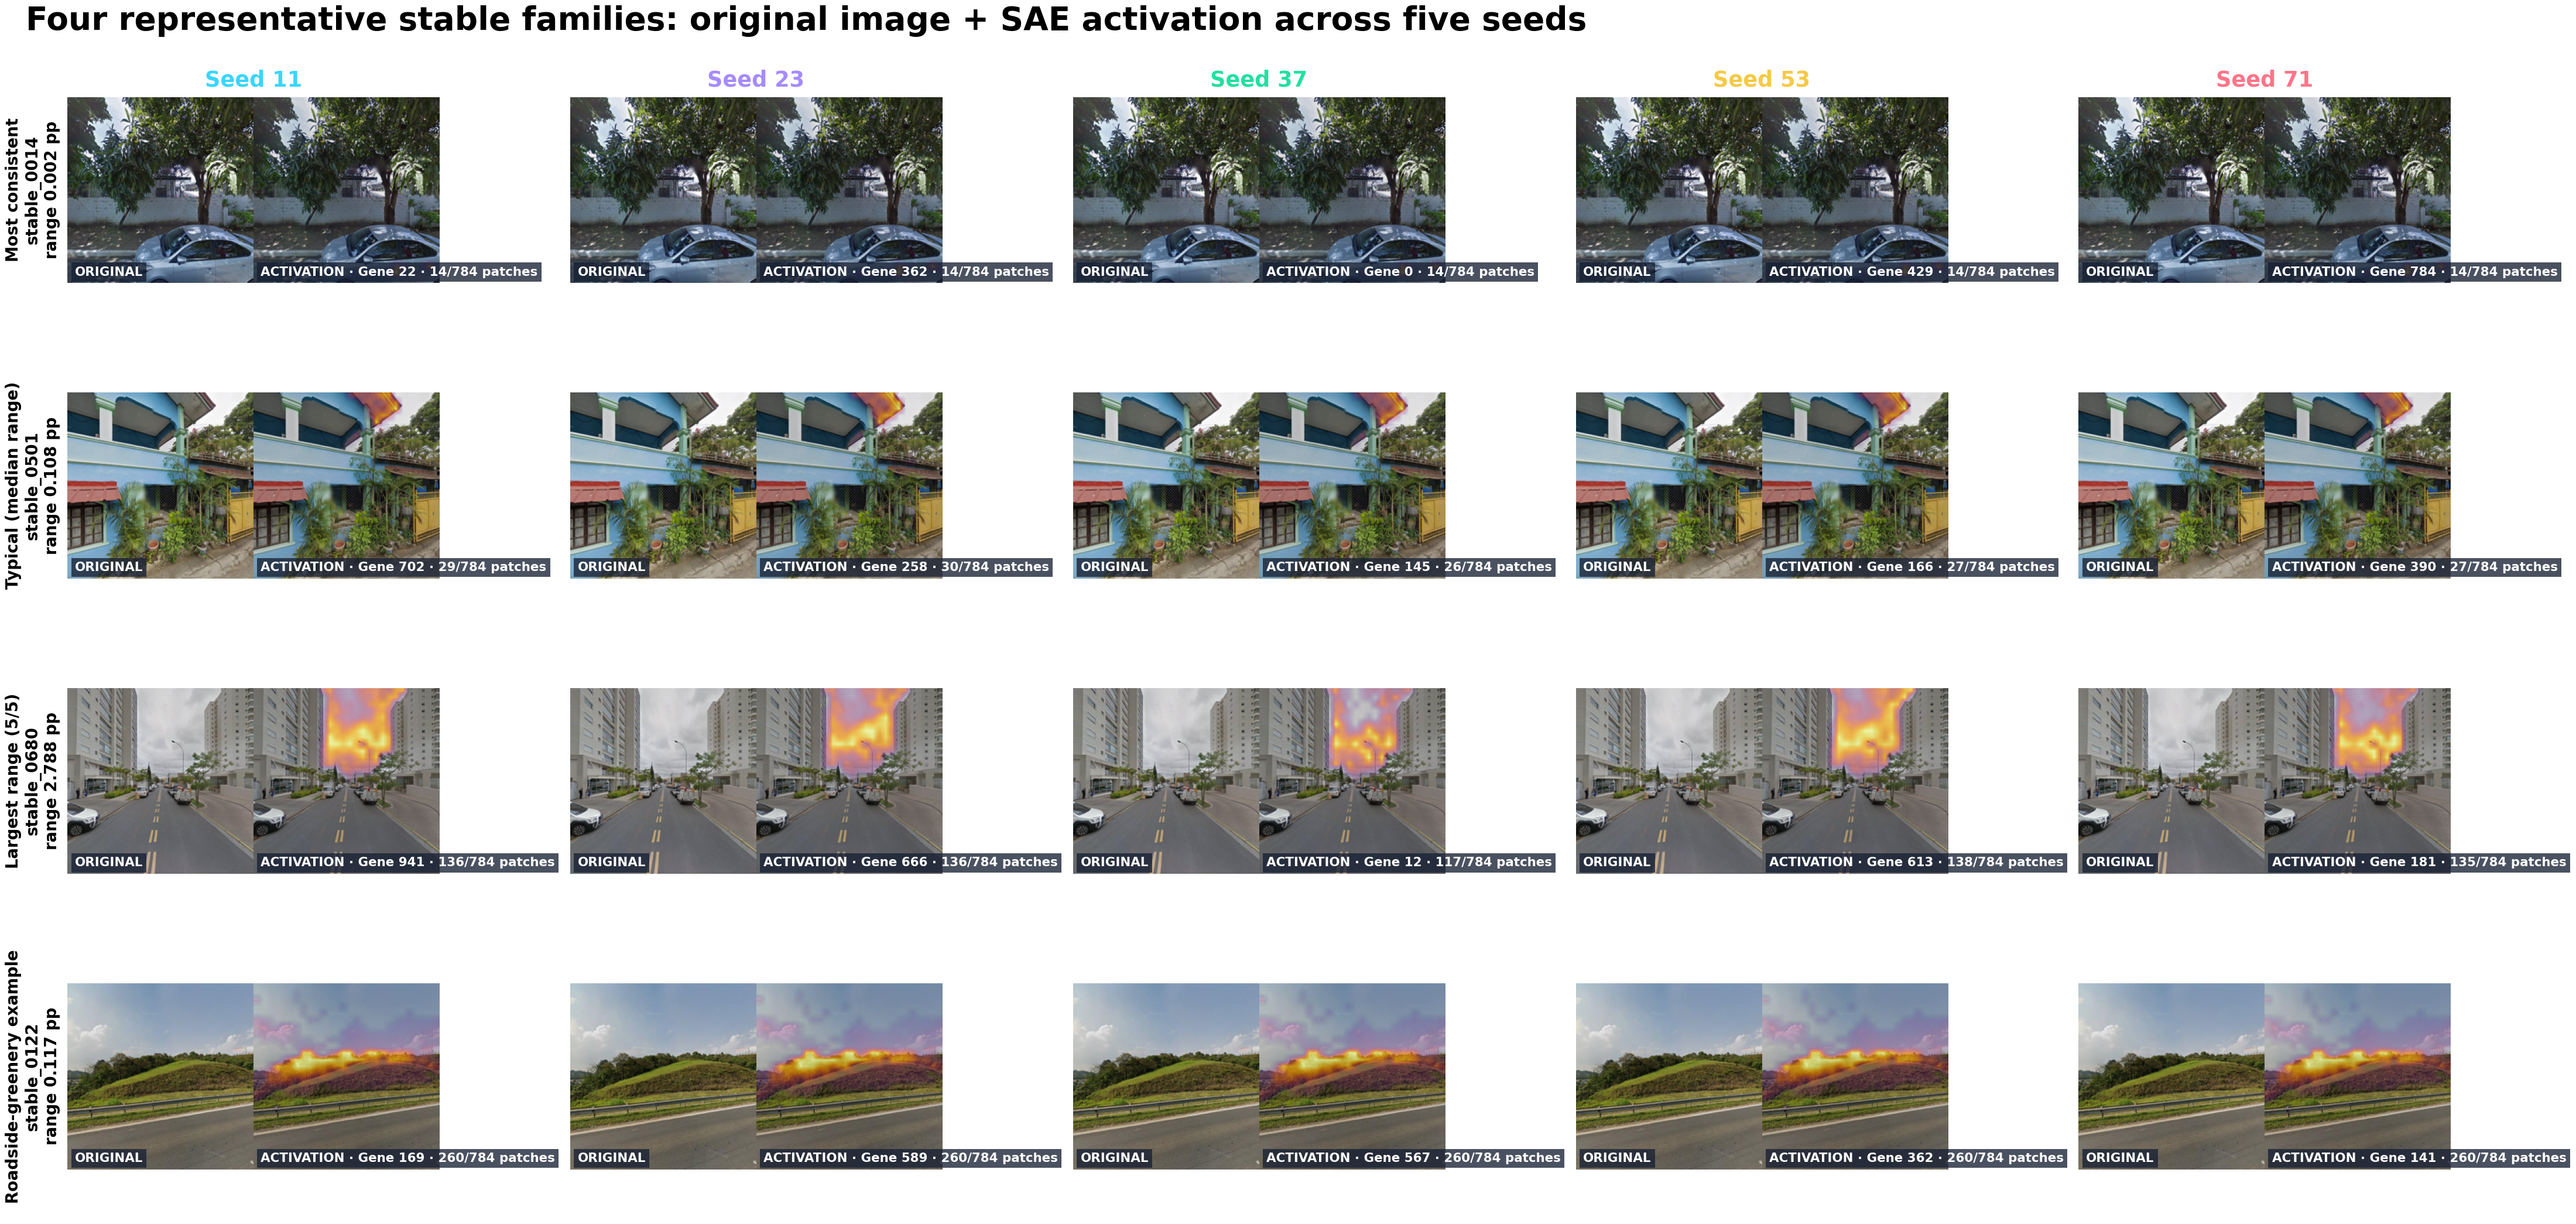
\includegraphics[width=\linewidth]{../formal/figures/sae_seed_representative_gene_montage.png}}{
\fbox{\parbox{0.9\linewidth}{\centering Missing figure: seed representative gene montage}}}
\caption{Representative cross-seed gene families. Features are matched using
decoder and held-out activation similarity rather than numeric gene IDs.}
\label{fig:stability}
\end{figure}

\subsection{Statistical taxonomy}
The fused graph is connected and supports 32 coarse and 64 fine branches. Evidence
roles include 251 stable structured genes, 107 city-specific components, 85 rare
stable components, 234 weakly structured components, 340 unstable components, two
position components, and five quality components. A stricter evidence audit finds
73 robust structured and 13 robust specific genes, while identifying 110 redundant
variants and seven nuisance components. Strict equivalence grouping suggests an
effective dictionary size of 932. These results show that the learned dictionary is
neither wholly semantic nor wholly noise: it mixes robust visual structure with
unstable, redundant, and acquisition-related directions.

\begin{figure}[t]
\centering
\IfFileExists{../formal/figures/taxonomy.png}{
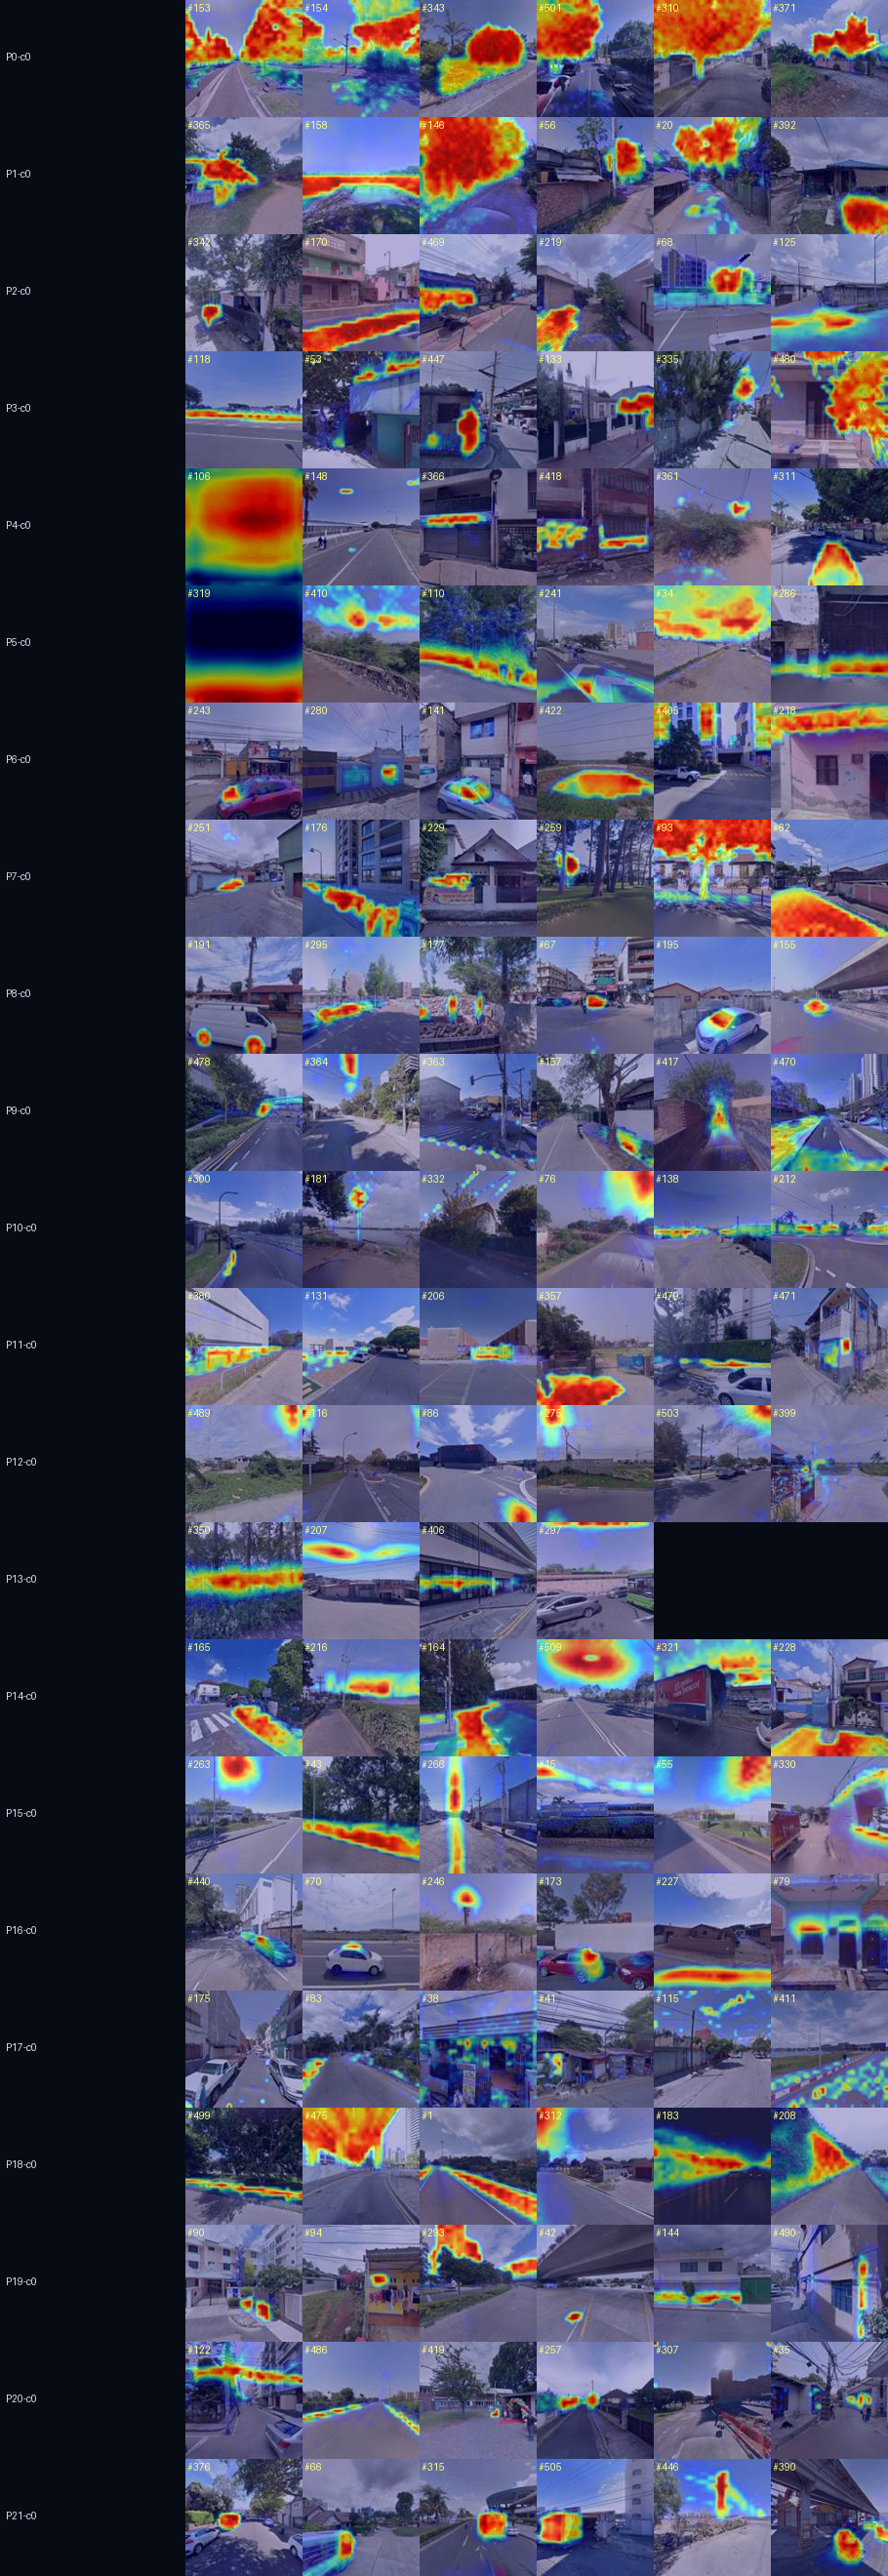
\includegraphics[width=0.95\linewidth,height=0.72\textheight,keepaspectratio]{../formal/figures/taxonomy.png}}{
\fbox{\parbox{0.9\linewidth}{\centering Missing figure: taxonomy}}}
\caption{Visual-gene organization. The displayed semantic categories are an
interpretive view; quantitative hierarchy selection itself uses no language labels.}
\label{fig:taxonomy}
\end{figure}

\subsection{External validity and nuisance controls}
Under five contiguous within-city spatial folds, gene profiles predict the nearest
road class with mean balanced accuracy 0.622 across 12 cities. This exceeds the class
prior (0.336) and nuisance-only features (0.388), and is comparable to dense DINO
features (0.616). Adding nuisance features to genes gives 0.620, suggesting that the
road signal is not explained by capture year, season, brightness, blur, sky fraction,
or QC flags alone.

For building targets in four cities, gene profiles show moderate average rank
association: Spearman $\rho=0.462$ for building coverage, 0.497 for log building
count, and 0.507 for distance to the nearest building. However, their mean held-out
$R^2$ values are strongly negative, indicating poor calibration and spatial
generalization under the current regression. Dense DINO features perform better in
$R^2$. We therefore treat building results as evidence of ordering information, not
accurate metric prediction.

For city classification over 3,600 panoramas, nuisance-only variables achieve 0.247
balanced accuracy, compared with 0.953 for gene profiles and 0.967 for dense DINO.
Residualizing nuisance variables changes gene accuracy only modestly (0.949).
Median cross-validated nuisance $R^2$ across genes is 0.010 (90th percentile 0.062),
although the most nuisance-predictable gene reaches 0.462. Nuisance control is thus
important at the feature level even when aggregate city prediction remains strong.

\subsection{Preliminary VLM interpretations}
Qwen returns valid structured JSON for all 128 pilot genes. The generated concept
types comprise 68 parts, 22 objects, 16 scenes, 10 artifacts, six textures, five
materials, and one layout. Examples include ``paved road surface'' (gene 405),
``man-made structure'' (gene 120), ``clear blue sky'' (gene 681), ``windowed
facade'' (gene 554), and ``delivery truck'' (gene 581). The average self-reported
confidence is 0.956, but the model marks no feature as a positional artifact even
though the statistical audit identifies position-related cases. This discrepancy
demonstrates why self-reported confidence is insufficient and motivates the held-out
fidelity experiment.

\section{Discussion}
The experiments support three conclusions. First, a sparse dictionary can retain
most of the local DINOv3 representation while exposing a compact set of activated
features. Second, much of this structure is reproducible across random
initializations, which is a stronger claim than interpretability from a single
training run. Third, gene distributions contain externally relevant urban-form
signal beyond simple acquisition and image-quality covariates.

At the same time, ``visual gene'' should not imply one feature equals one clean human
concept. Some dimensions are broad, redundant, unstable, positional, or related to
image quality. The VLM pilot makes the output easier to browse but also reveals a
failure mode: fluent, high-confidence descriptions can miss statistically diagnosed
artifacts. A defensible release should therefore expose evidence scores and
counterexamples alongside every natural-language label.

\section{Limitations and Next Steps}
\begin{itemize}[leftmargin=*]
  \item The reported SAE is trained on 12 cities; claims about the 110-city corpus
  require global encoding and geographically held-out evaluation.
  \item The current main experiment treats patches as observations, but a controlled
  comparison against global embeddings, four-view means, separate directional views,
  and concatenated views remains unfinished because of cluster-environment failures.
  \item The VLM pilot lacks independent fidelity scores. We will ask a separate judge
  (and a blinded human subset) whether generated concepts distinguish held-out
  positive from matched negative examples.
  \item Gene matching uses fixed similarity thresholds. Sensitivity analysis and
  uncertainty intervals are needed.
  \item External building prediction is poorly calibrated under spatial folds;
  downstream interpretation should emphasize rank association until improved.
  \item Google Street View sampling, geographic coverage, temporal variation, and
  platform-specific artifacts can bias cross-city comparisons.
\end{itemize}

\section{Conclusion}
\method{} turns dense patch representations into a sparse, auditable vocabulary for
comparative urban imagery. The present evidence establishes reconstruction,
cross-seed reproducibility, statistical organization, and partial external validity.
The next scientific priority is not simply scaling the dictionary, but validating
which individual genes have faithful semantic interpretations and remain robust
across cities, time, position, and acquisition conditions.

\paragraph{Data and code availability.}
An interactive research dashboard is available at
\url{https://cehougis.github.io/urban-visual-gene/}. \todo{Add an archival code
release, model checkpoint license, street-view redistribution statement, and DOI.}

\paragraph{Acknowledgments.}
\todo{Add collaborators, funding, Savio/BRC acknowledgement, and data-provider
acknowledgments.}

\bibliographystyle{plain}
\bibliography{references}

\appendix
\section{Current project status}
As of September 2026, the main W1024/K8 model, width/sparsity ablations, five-seed
matching, statistical taxonomy, external-validity analysis, nuisance controls, and
128-gene Qwen labeling run are complete. The controlled observation-unit ablation
and independent VLM fidelity evaluation remain incomplete. This appendix is a draft
status record and should be removed or updated before submission.

\end{document}
